\documentclass[letter,twoside,11pt]{article}

\usepackage[spanish,es-nodecimaldot]{babel}
\usepackage[utf8]{inputenc}

\usepackage{lmodern}
\usepackage[T1]{fontenc}
\usepackage{textcomp}

\usepackage{framed}
\usepackage[svgnames]{xcolor}
\colorlet{shadecolor}{Gainsboro!50}

\usepackage[labelfont=bf]{caption}
\usepackage{graphicx}
\usepackage{pstricks}

\usepackage{anysize}
\marginsize{3cm}{2cm}{2cm}{3cm}

\usepackage{siunitx}
\usepackage{amsmath}
\usepackage{array}
\usepackage{csquotes}

\usepackage{fancyhdr}
\usepackage{lastpage}
\pagestyle{fancy}
\fancyhf{}
\fancyhead[LE,RO]{Laboratorio de Electrónica Analógica I}
\fancyfoot[CO,CE]{\thepage\ de \pageref{LastPage}}

\special{papersize=215.9mm,279.4mm}

\usepackage[
    pdfauthor={Carlos Eduardo Caballero Burgoa},%
    pdftitle={Laboratorio de Electrónica Analógica I},%
    pdfsubject={Curva de polarización de un diodo. Circuitos recortadores y
    sustentadores},%
    colorlinks,%
    citecolor=black,%
    filecolor=black,%
    linkcolor=black,%
    urlcolor=black,
    breaklinks]{hyperref}
\usepackage{breakurl}

\newcommand{\blankpage}{
\newpage
\thispagestyle{empty}
\mbox{}
\newpage
}

\renewcommand{\arraystretch}{1.2}

\begin{document}

\begin{titlepage}
    \begin{center}
        {\Large UNIVERSIDAD MAYOR DE SAN SIMÓN}\\
        \vspace*{0.15cm}
        {\large FACULTAD DE CIENCIAS Y TECNOLOGÍA}\\
        \vspace*{0.10cm}
        DEPARTAMENTO DE ELÉCTRICA-ELECTRÓNICA\\
        \vspace*{3.0cm}
        {\Large \textbf{LABORATORIO DE ELECTRÓNICA ANALÓGICA I}}\\
        \vspace*{0.3cm}
        {\Large \textbf{INFORME No. 1}}\\
        \vspace*{3.5cm}
        {\Large \textbf{CURVA DE POLARIZACIÓN DE UN DIODO.\\
        CIRCUITOS RECORTADORES Y SUSTENTADORES}}\\
    \end{center}

    \vspace*{5.8cm}
    \leftskip=7.95cm
    \noindent
    \textbf{Estudiante:}\\
    Caballero Burgoa, Carlos Eduardo.\\
    \newline
    \textbf{Carrera:}\\
    Ing. Electromecánica.\\
    \newline
    \textbf{Docente:}\\
    Ing. Alberto Arispe Santander.\\
    \newline
    \textbf{Grupo:} 1B.\\
    \textbf{Fecha de entrega:} 8 de Octubre del 2024.\\
\end{titlepage}

\section{Introducción}
El dispositivo electrónico no lineal más simple se conoce como \emph{diodo}. Un
diodo está compuesto de dos materiales diferentes (unión \emph{pn}) colocados
juntos de tal forma que la carga fluye fácilmente en una dirección, pero no en
dirección contraria. El comportamiento del diodo depende de la polaridad de la
tensión aplicada.

Para polarizar un diodo se aplica un voltaje de corriente continua a través de
él. La \textbf{polarización en directa} es la condición que permite la
circulación de corriente a través de la unión \emph{pn}. La \textbf{polarización
en inversa} es la condición que en esencia evita la circulación de corriente a
través del diodo \cite{Floyd}.

Los diodos tienen muchas aplicaciones, entre ellas están las de recortar una
señal de entrada o limitar solo partes de la señal. Además se pueden utilizar
para restablecer un nivel de corriente directa a una señal de entrada.

Los circuitos \textbf{recortadores} se utilizan para eliminar parte de una forma
de onda que se encuentre por encima o por debajo de algún nivel de referencia.
Los circuitos recortadores se conocen a veces como: limitadores, selectores de
amplitud o rebanadores.

Una forma de onda de tensión se puede desplazar añadiendo en serie con ella una
fuente de tensión independiente, ya sea constante o dependiente del tiempo. La
fijación o \textbf{sustentación} es una operación de desplazamiento, pero la
cantidad de éste depende de la forma de la onda real \cite{Savant}.

\section{Objetivos}
\begin{itemize}
    \item Verificar la curva característica de polarización de un diodo.
    \item Verificar el comportamiento de los circuitos recortadores.
    \item Verificar el comportamiento de los circuitos sustentadores.
\end{itemize}

\section{Marco Teórico}

\subsection{Curva característica de polarización}
En la \textbf{figura~\ref{curva}}, se muestra la gráfica de la corriente a
través del diodo en función del voltaje de entrada; donde pueden observarse tres
regiones donde puede operar un diodo \cite{Tancara}:

\begin{figure}[!h]
\centering
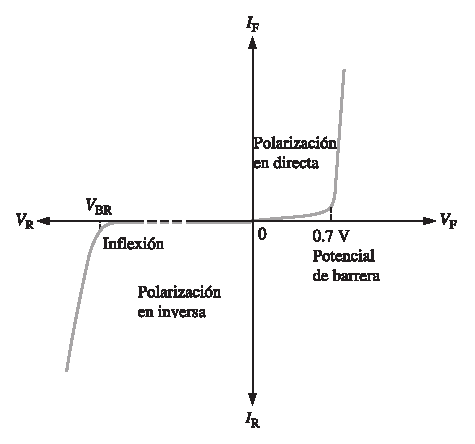
\includegraphics[scale=1.10]{figura1.eps}
\caption{Curva característica $V-I$ para un diodo.}
\label{curva}
\end{figure}

\begin{description}
    \item [Región de conducción en polarización directa (PD):]
        Donde $V_D \text{(Potencial de barrera)} > 0[\text{V}]$, siendo:
        \begin{itemize}
            \item La corriente en el diodo muy pequeña, cuando:
                $0[\text{V}] < V_D < V_F$.
            \item La corriente en el diodo es cada vez mas grande, cuando:
                $V_D > V_F$.
        \end{itemize}
    \item [Región de no conducción:]
        Donde $V_D < 0[\text{V}]$, siendo la corriente en el diodo demasiado
        pequeña y negativa, conocida como corriente de saturación inversa:
        $I_S$.
    \item [Región de conducción en polarización inversa:]
        Se encuentra a la izquierda del voltaje de ruptura ($V_{BR}$), para
        voltajes del diodo cada vez mayor, pero negativo, el diodo se encuentra
        con corriente cada vez mas grande (pero negativa), conocida como
        corriente de avalancha.
\end{description}

\subsection{Circuito recortador}
Este tipo de circuito permite obtener en la salida una fracción de la señal de
entrada, como si hubiese sufrido un recorte. Se emplean para eliminar una parte
de la forma de onda que se encuentra por encima o por debajo de algún nivel de
referencia deseado. La señal de entrada puede tener cualquier forma de onda;
dependiendo de los componentes y de la forma en que se encuentren conectados
entre si, el circuito recortador puede actuar de diferente forma sobre la señal
de entrada.

Mínimamente deberá contar con un resistor y un diodo, para que el recorte se
realice a partir de la referencia (en las proximidades de $0[\text{V}]$
eliminando la parte superior o inferior, dependiendo de la orientación del
diodo. Si se agrega una fuente de voltaje, la referencia para el recorte puede
quedar desplazada, hacia arriba o hacia abajo \cite{Tancara}.

En la \textbf{figura~\ref{recortador1}} puede verse la señal de entrada y la
señal de salida para un circuito recortador sin una fuente de voltaje adicional.

\begin{figure}[!h]
\centering
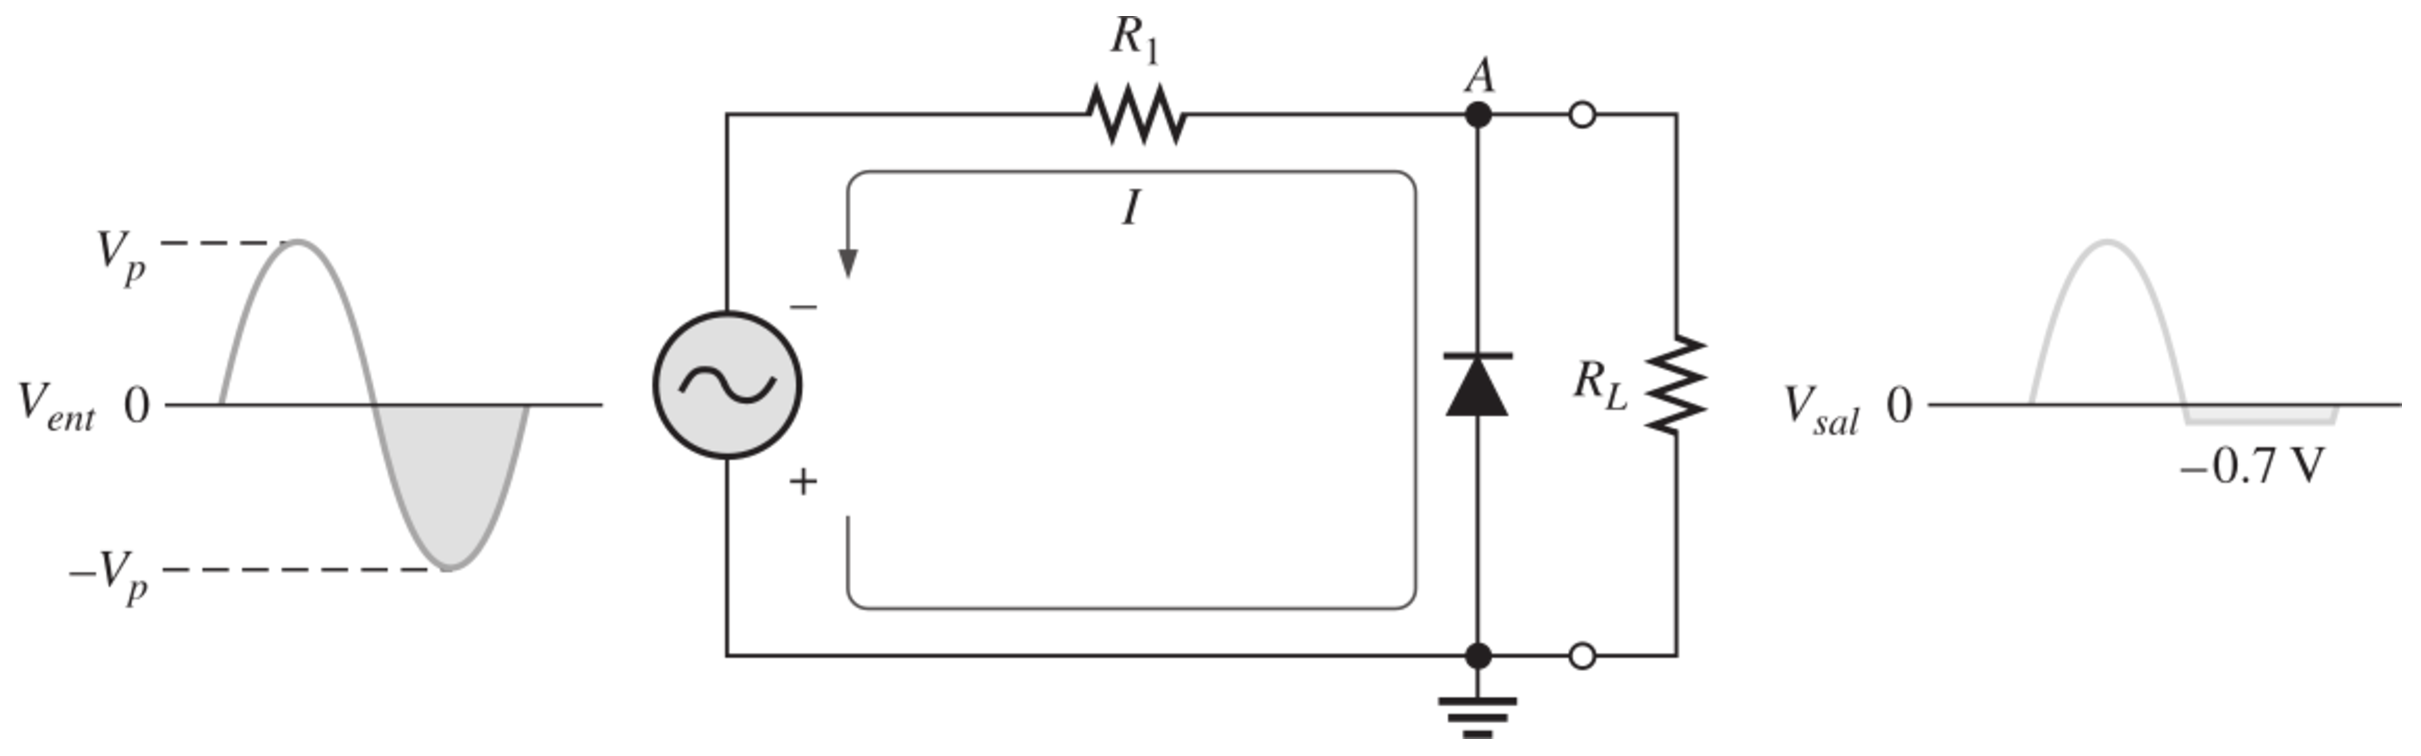
\includegraphics[scale=0.29]{figura2.eps}
\caption{Circuito recortador sin fuente de voltaje.}
\label{recortador1}
\end{figure}

En la \textbf{figura~\ref{recortador2}} puede verse la señal de entrada y la
señal de salida para un circuito recortador que posee una fuente de voltaje
adicional que sube el valor mínimo de la salida una cantidad predeterminada.

\begin{figure}[!h]
\centering
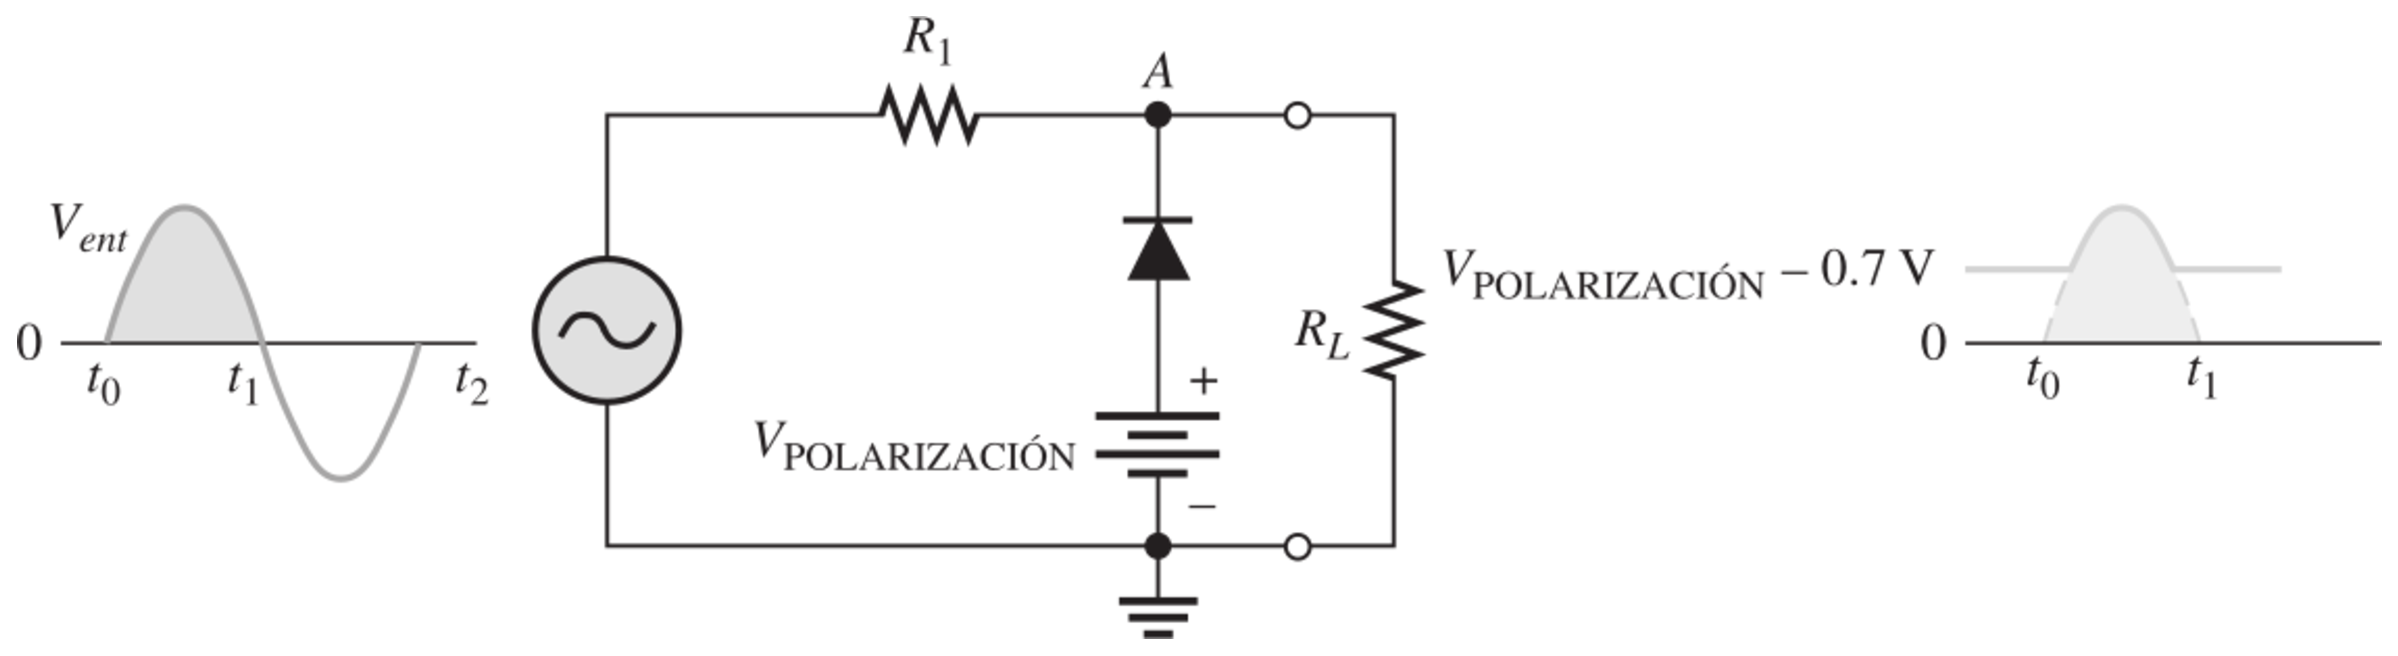
\includegraphics[scale=0.28]{figura3.eps}
\caption{Circuito recortador con fuente de voltaje.}
\label{recortador2}
\end{figure}

\subsection{Circuito sustentador}
Este tipo de circuito permite obtener en la salida la misma señal de entrada
pero desplazada, ya sea hacia arriba o hacia abajo. La señal de entrada puede
tener cualquier forma de onda. Mínimamente deberá contar con un capacitor, un
resistor y un diodo. Si se agrega una fuente de voltaje, la sustentación puede
ser mas pronunciada \cite{Tancara}.

En la \textbf{figura~\ref{fijador1}} puede verse la señal de entrada y la señal
de salida para un circuito sustentador sin una fuente de voltaje adicional.

\begin{figure}[!h]
\centering
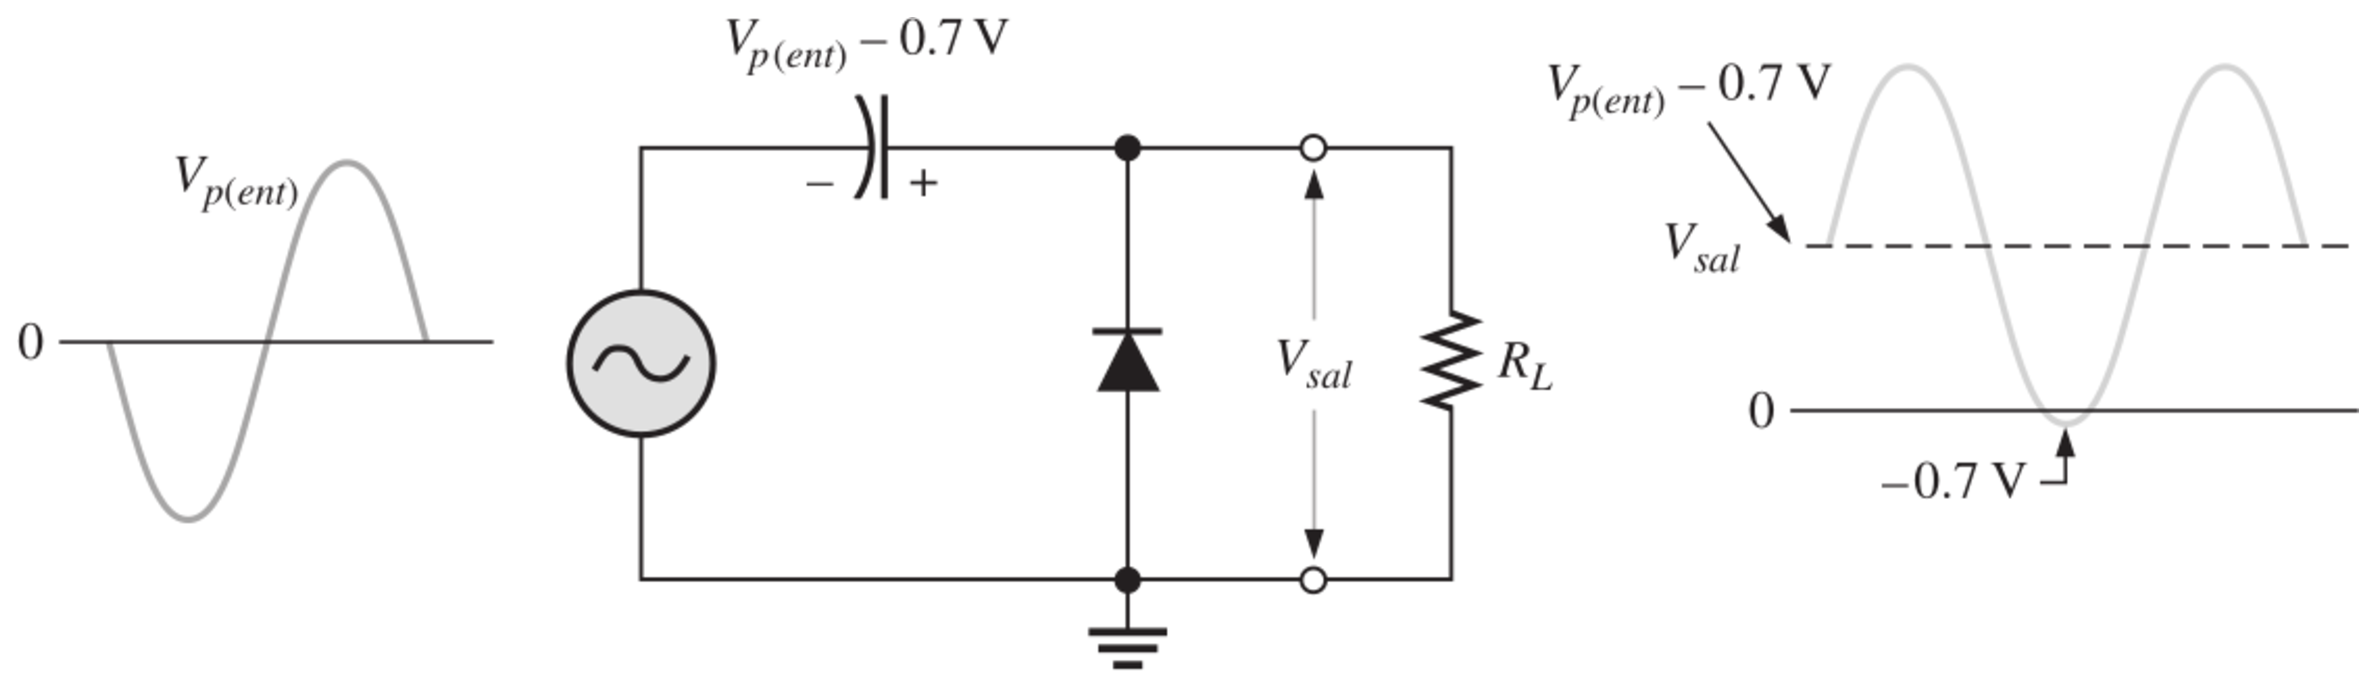
\includegraphics[scale=0.30]{figura4.eps}
\caption{Circuito sustentador sin fuente de voltaje.}
\label{fijador1}
\end{figure}

\section{Simulación}
Se utilizó el software \emph{Quite Universal Circuit Simulator.} versión 23.3.1
para simular los circuitos.

\subsection{Curva de polarización}
Para la simulación y el experimento se utilizan los siguientes componentes:

\begin{itemize}
    \item Dos diodos rectificadores 1N4001 50V 1A.
    \item Una placa de pruebas.
    \item Un voltímetro.
    \item Un amperímetro.
    \item Fuente de alimentación $DC$.
    \item Cable conector para la fuente de alimentación $DC$.
    \item Cables de conexión.
\end{itemize}

La curva característica simulada para dos diodos en serie puede verse en la
\textbf{figura~\ref{simulacion1}}, en esta puede apreciarse la gráfica de
corriente en función del voltaje de entrada, además de la gráfica de voltaje de
los diodos en serie en función del voltaje de entrada.

\begin{figure}[!h]
\centering
\includegraphics[scale=0.97]{simulacion/practica1.1.eps}
\caption{Simulación de la curva V-I en dos diodos en serie.}
\label{simulacion1}
\end{figure}

\subsection{Circuitos recortadores}
Para la simulación y el experimento se utilizan los siguientes componentes:

\begin{itemize}
    \item Un diodo rectificador 1N4001 50V 1A.
    \item Una resistencia $10\,[k\Omega]$.
    \item Una placa de pruebas.
    \item Generador de funciones.
    \item Osciloscopio.
    \item Fuente de alimentación $DC$.
    \item Cable conector para la fuente de alimentación $DC$.
    \item Dos cables BNC para conexión del generador de funciones.
    \item Cables de conexión.
\end{itemize}

\subsubsection{Recortador sin fuente de voltaje}
Se simulo un circuito recortador con tres tipos diferentes de señales: una señal
rectangular (\textbf{figura~\ref{simulacion2}}), una señal triangular
(\textbf{figura~\ref{simulacion3}}) y una señal senoidal
(\textbf{figura~\ref{simulacion4}}).

\begin{figure}[!h]
\centering
\includegraphics[scale=0.97]{simulacion/practica1.2.eps}
\caption{Simulación de un recortador con una señal rectangular.}
\label{simulacion2}
\end{figure}

\begin{figure}[!h]
\centering
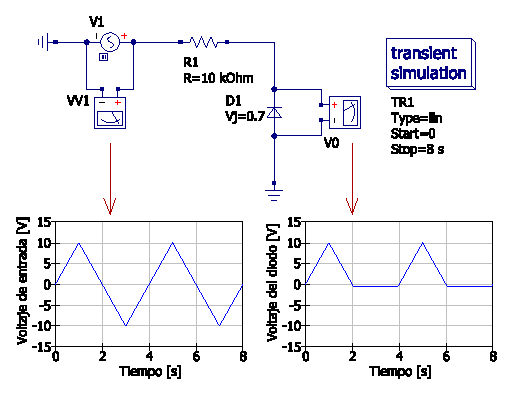
\includegraphics[scale=0.97]{simulacion/practica1.3.eps}
\caption{Simulación de un recortador con una señal triangular.}
\label{simulacion3}
\end{figure}

\begin{figure}[!h]
\centering
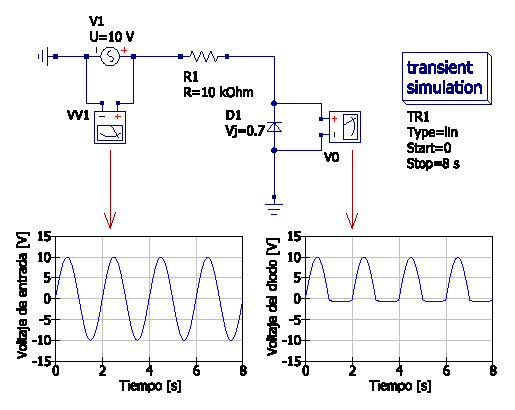
\includegraphics[scale=0.97]{simulacion/practica1.4.eps}
\caption{Simulación de un recortador con una señal senoidal.}
\label{simulacion4}
\end{figure}

\subsubsection{Recortador con fuente de voltaje}
Se simulo un circuito recortador con fuente de voltaje de $5[\text{V}]$ con tres
tipos diferentes de señales: una señal rectangular
(\textbf{figura~\ref{simulacion5}}), una señal triangular
(\textbf{figura~\ref{simulacion6}}) y una señal senoidal
(\textbf{figura~\ref{simulacion7}}), en la gráfica de salida de la señal puede
verse el valor mínimo subido hasta los $5[\text{V}]$ menos el voltaje de
polarización del diodo.

\begin{figure}[!h]
\centering
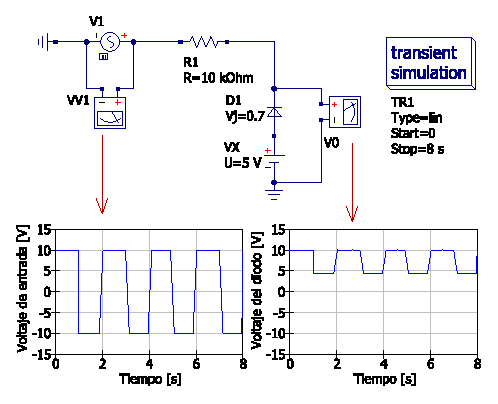
\includegraphics[scale=0.97]{simulacion/practica1.5.eps}
\caption{Simulación de un recortador con fuente de voltaje con una señal
rectangular.}
\label{simulacion5}
\end{figure}

\begin{figure}[!h]
\centering
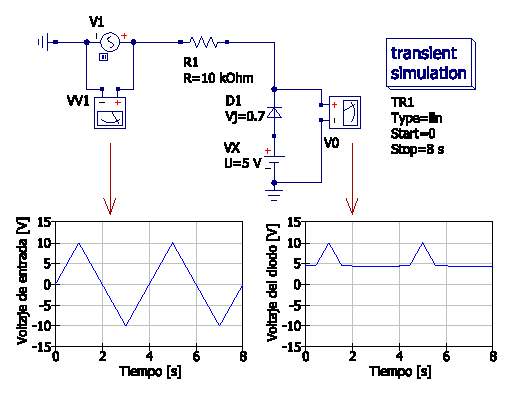
\includegraphics[scale=0.97]{simulacion/practica1.6.eps}
\caption{Simulación de un recortador con fuente de voltaje con una señal
triangular.}
\label{simulacion6}
\end{figure}

\begin{figure}[!h]
\centering
\includegraphics[scale=0.97]{simulacion/practica1.7.eps}
\caption{Simulación de un recortador con fuente de voltaje con una señal
senoidal.}
\label{simulacion7}
\end{figure}

\subsection{Circuitos sustentadores}
Para la simulación y el experimento se utilizan los siguientes componentes:

\begin{itemize}
    \item Un diodo rectificador 1N4001 50V 1A.
    \item Una resistencia $10\,[k\Omega]$.
    \item Un capacitor $470\,[\mu F]$.
    \item Una placa de pruebas.
    \item Generador de funciones.
    \item Osciloscopio.
    \item Fuente de alimentación $DC$.
    \item Cable conector para la fuente de alimentación $DC$.
    \item Dos cables BNC para conexión del generador de funciones.
    \item Cables de conexión.
\end{itemize}

\subsubsection{Sustentador sin fuente de voltaje}
Se simulo un circuito sustentador con tres tipos diferentes de señales: una
señal rectangular (\textbf{figura~\ref{simulacion8}}), una señal triangular
(\textbf{figura~\ref{simulacion9}}) y una señal senoidal
(\textbf{figura~\ref{simulacion10}}).

\begin{figure}[!h]
\centering
\includegraphics[scale=0.97]{simulacion/practica1.8.eps}
\caption{Simulación de un sustentador con una señal rectangular.}
\label{simulacion8}
\end{figure}

\begin{figure}[!h]
\centering
\includegraphics[scale=0.97]{simulacion/practica1.9.eps}
\caption{Simulación de un sustentador con una señal triangular.}
\label{simulacion9}
\end{figure}

\begin{figure}[!h]
\centering
\includegraphics[scale=0.97]{simulacion/practica1.10.eps}
\caption{Simulación de un sustentador con una señal senoidal.}
\label{simulacion10}
\end{figure}

\subsubsection{Sustentador con fuente de voltaje}
Se simulo un circuito sustentador con fuente de voltaje de $5[\text{V}]$ con
tres tipos diferentes de señales: una señal rectangular
(\textbf{figura~\ref{simulacion11}}), una señal triangular
(\textbf{figura~\ref{simulacion12}}) y una señal senoidal
(\textbf{figura~\ref{simulacion13}}).

\begin{figure}[!h]
\centering
\includegraphics[scale=0.97]{simulacion/practica1.11.eps}
\caption{Simulación de un sustentador con fuente de voltaje con una señal
rectangular.}
\label{simulacion11}
\end{figure}

\begin{figure}[!h]
\centering
\includegraphics[scale=0.97]{simulacion/practica1.12.eps}
\caption{Simulación de un sustentador con fuente de voltaje con una señal
triangular.}
\label{simulacion12}
\end{figure}

\begin{figure}[!h]
\centering
\includegraphics[scale=0.97]{simulacion/practica1.13.eps}
\caption{Simulación de un sustentador con fuente de voltaje con una señal
senoidal.}
\label{simulacion13}
\end{figure}

\newpage
\section{Resultados}

\subsection{Curva de polarización}
Una vez montado el experimento en laboratorio se obtuvieron los siguientes
valores:

\begin{center}
    \begin{tabular}{|c|c|c|}
    \hline
    $V_i[\text{V}]$ & $V_d[\text{V}]$ & $i[\text{A}]$
    \tabularnewline \hline \hline
    $0.4$ & $0.29$ & $0.001$ \tabularnewline \hline
    $1$   & $0.80$ & $0.014$ \tabularnewline \hline
    $2$   & $0.95$ & $0.094$ \tabularnewline \hline
    $3$   & $1.02$ & $0.188$ \tabularnewline \hline
    $4$   & $1.06$ & $0.286$ \tabularnewline \hline
    $5$   & $1.08$ & $0.379$ \tabularnewline \hline
    \end{tabular}
\end{center}

Cuya gráfica $V-I$ se presenta en la \textbf{figura~\ref{grafica}}:

\begin{figure}[!h]
\centering
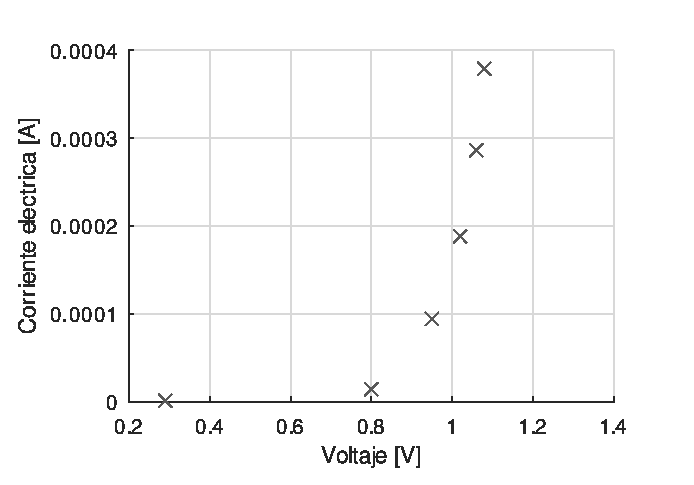
\includegraphics[scale=0.75]{graficas/o1.eps}
\caption{Curva característica $V-I$ para dos diodos 1N4001 en serie.}
\label{grafica}
\end{figure}

\subsection{Circuitos recortadores}
En la \textbf{figura~\ref{labo1}} se presenta el montaje del circuito
recortador simulado con los componentes descritos en la sección anterior.

\begin{figure}[!h]
\centering
\includegraphics[scale=0.10]{fotos/labo1.1.eps}
\caption{Montaje del circuito recortador.}
\label{labo1}
\end{figure}

\subsubsection{Recortador sin fuente de voltaje}
En la \textbf{figura~\ref{labo2}} se presentan las salidas del osciloscopio para
el voltaje de entrada y el voltaje de salida para las señales rectangular,
triangular y senoidal respectivamente.

\begin{figure}[!h]
\centering
\includegraphics[scale=0.077]{fotos/labo1.2.eps}
\includegraphics[scale=0.070]{fotos/labo1.3.eps}
\includegraphics[scale=0.070]{fotos/labo1.4.eps}
\caption{Salida del osciloscopio para diferentes señales de entrada.}
\label{labo2}
\end{figure}

\subsubsection{Recortador con fuente de voltaje}
En la \textbf{figura~\ref{labo3}} se presentan las salidas del osciloscopio para
el voltaje de entrada y el voltaje de salida para las señales rectangular,
triangular y senoidal respectivamente.

\begin{figure}[!h]
\centering
\includegraphics[scale=0.071]{fotos/labo1.5.eps}
\includegraphics[scale=0.069]{fotos/labo1.6.eps}
\includegraphics[scale=0.068]{fotos/labo1.7.eps}
\caption{Salida del osciloscopio para diferentes señales de entrada.}
\label{labo3}
\end{figure}

\subsection{Circuitos sustentadores}
En la \textbf{figura~\ref{labo4}} se presenta el montaje del circuito
sustentador simulado con los componentes descritos en la sección anterior.

\begin{figure}[!h]
\centering
\includegraphics[scale=0.117]{fotos/labo1.8.eps}
\caption{Montaje del circuito sustentador.}
\label{labo4}
\end{figure}

\subsubsection{Sustentador sin fuente de voltaje}
En la \textbf{figura~\ref{labo5}} se presentan las salidas del osciloscopio para
el voltaje de entrada y el voltaje de salida para las señales rectangular,
triangular y senoidal respectivamente.

\begin{figure}[!h]
\centering
\includegraphics[scale=0.055]{fotos/labo1.9.eps}
\includegraphics[scale=0.065]{fotos/labo1.10.eps}
\includegraphics[scale=0.096]{fotos/labo1.11.eps}
\caption{Salida del osciloscopio para diferentes señales de entrada.}
\label{labo5}
\end{figure}

\subsubsection{Sustentador con fuente de voltaje}
En la \textbf{figura~\ref{labo6}} se presentan las salidas del osciloscopio para
el voltaje de entrada y el voltaje de salida para las señales rectangular,
triangular y senoidal respectivamente.

\begin{figure}[!h]
\centering
\includegraphics[scale=0.073]{fotos/labo1.12.eps}
\includegraphics[scale=0.080]{fotos/labo1.13.eps}
\includegraphics[scale=0.102]{fotos/labo1.14.eps}
\caption{Salida del osciloscopio para diferentes señales de entrada.}
\label{labo6}
\end{figure}

\section{Conclusiones y Recomendaciones}
Se comprobó que los comportamientos tanto de la curva característica del diodo,
como de los circuitos recortadores y sustentadores, son similares en la teoría,
la simulación y experimentalmente.

Se constato que los instrumentos provistos en el laboratorio (fuentes de
alimentación DC, generador de funciones y osciloscopio) son vitales en el
análisis de circuitos y lo importante que es conocer todas las funciones que
proveen estos.

A su vez, de los componentes electrónicos de los diferentes circuitos armados
es crucial hacer una revisión de sus hojas de datos, para evitar que el diseño
exceda sus valores recomendados de funcionamiento.

\begin{thebibliography}{99}

\bibitem{Floyd}
Thomas L. Floyd (208).\\
\textbf{Dispositivos electrónicos. 8va Edición.}\\
Pearson Education

\bibitem{Savant}
C.J. Savant Jr, Martin S. Roden, Gordon Carpenter. (1992).\\
\textbf{Diseño Electrónico. Circuitos y sistemas. 2da Edición.}\\
Addison-Wesley

\bibitem{Tancara}
Ing. Jose F. Tancara S. (2019).\\
\textbf{Guía de laboratorio electrónica analógica I}\\

\end{thebibliography}

\end{document}

